\subsection*{選択テーマ}
本実験でFPGA上で実装するテーマとして、巡回セールスマン問題を選択した。
いくつかあるバリエーションのうち、本実験では、以下のように問題設定を行った。
\begin{itembox}[l]{問題設定}
    256×256のマス目上に、ランダムに配置された64個の点がある。
    これらの点をすべてめぐって元の点に戻ってくるような閉路(ハミルトン閉路)のうち、
    総距離ができるだけ小さいものを求めよ。
\end{itembox}
例えば、図\ref{fig:tspsapmle}においては、右図は左図に比べ総距離が小さく評価が高い。
\begin{figure}[h]
    \label{fig:tspsapmle}
    \begin{center}
        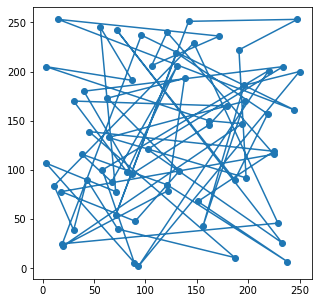
\includegraphics[width=7cm]{figure/tsp_bad.png}
        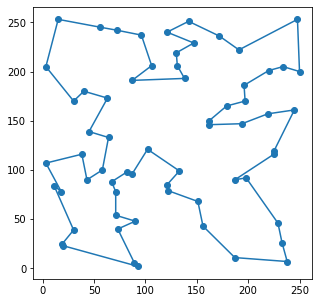
\includegraphics[width=7cm]{figure/tsp_good.png}
        \caption{
            今回の問題設定における巡回セールスマン問題の例\\
            (左) 総距離が大きい経路(総距離: 8437.0)
            (右) 総距離が小さい経路(総距離: 1748.6)
        }
    \end{center}
\end{figure}
\subsection*{背景: 巡回セールスマン問題の解法}
巡回セールスマン問題は、NP困難であることが知られている。つまり、厳密な最適解を多項式時間で求めることはできない。
頂点数が20程度の小さな問題であれば動的計画法によって最適解を求めることができるが、それ以上の規模ではヒューリスティックな手法を用いて最適解に近づける手法が主となる。
ヒューリスティックな手法の多くは、局所探索法の考え方に基づいている。
\subsubsection*{局所探索法}\label{sec:local}
局所探索法とは、ある解から出発して、その近傍解(一部を変えた解)を探索することを繰り返すことで、最適解に近づける手法である。
近傍解の生成方法には様々な種類があり、それぞれ最適解へのたどり着きやすさ・生成に要する時間・並列可能性などの特徴が異なる。
そのうち最もシンプルな方法が、経路のうち2つの頂点を入れ替えることで近傍解を生成する方法である。
例えば、図\ref{fig:tspswap}において、元々の経路(左図)の一部に1→5→3という部分と4→2→6という部分があったとき、右図のように1→2→3と4→5→6という経路に変更することで近傍解を生成する。
この変更は、経路の2と5を入れ替えることで実現でき、生成にかかるコストが非常に低い。また、この方法は並列可能性がとても高い。
二点を入れかえるべきかどうかを計算するには、入れかえる2点と、それぞれの前後の点の計6点の情報がわかっていれば良い。
これら6点が重複しないように選択すれば、複数の箇所について同時に近傍を生成し、判定・更新を行うことができる。
例えば図~\ref{fig:tspswapparallel}において、青で示した部分と赤で示した部分は独立に判定・更新可能である。
\begin{figure}[h]
    \label{fig:tspswap}
    \begin{center}
        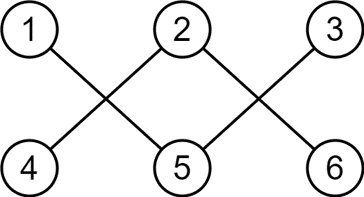
\includegraphics[width=6cm]{figure/swap_bad.png}
        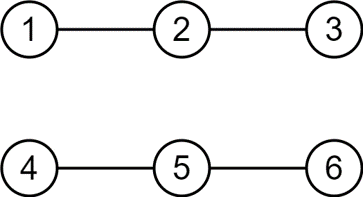
\includegraphics[width=6cm]{figure/swap_good.png}
        \caption{
            (左)交換前の経路[1→5→3 / 4→2→6]
            (右)交換後の経路[1→2→3 / 4→5→6]
        }
    \end{center}
\end{figure}

\begin{figure}[h]
    \label{fig:tspswapparallel}
    \begin{center}
        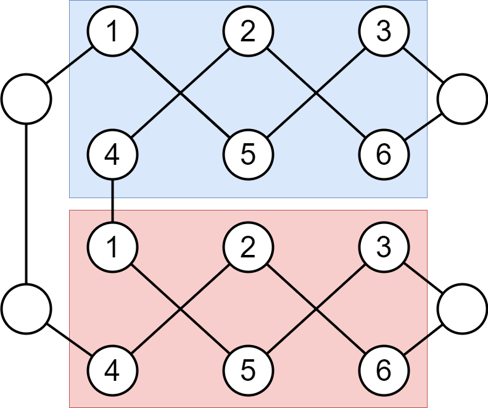
\includegraphics[width=6cm]{figure/parallel_swap_bef.png}
        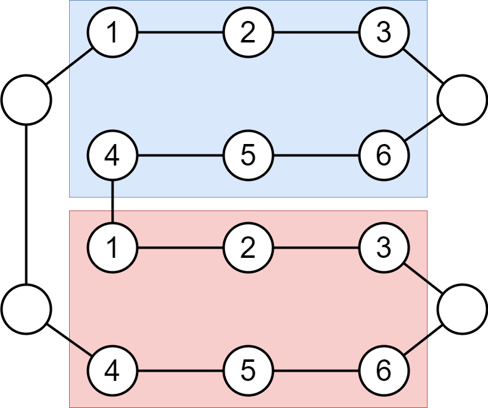
\includegraphics[width=6cm]{figure/parallel_swap_aft.png}
        \caption{
            複数の箇所について同時に近傍を生成し、判定・更新を行う例
        }
    \end{center}
\end{figure}

ランダムな近傍を繰り返し生成し、総距離が小さくなるような近傍を見つけたら、貪欲にその近傍に移動することを繰り返すことで、最適解に近づける方法を山登り法と呼ぶ。

\subsubsection*{山登り法のデメリットとその対策}
山登り法は、局所最適解に陥りやすいという欠点がある。
局所最適解とは、ある解の近傍にあるいずれの解によっても結果が改善しない解のことである。これは必ずしも最適解とは限らない。

結果が改善する近傍のみを採用する山登り法では、局所最適解に陥ると、そこから脱出することができなくなる。この問題に対しては以下のような手法が存在する。
\begin{itemize}
    \item 焼き鈍し法: 結果が改善する近傍を必ず採用することに加え、結果が改善しない近傍も一定の確率で採用することで、局所最適解に陥りにくくする手法
    \item 反復局所探索法: 山登り法によって局所最適解に陥ったら解の一部分を崩す、という操作を繰り返すことで、局所最適解に陥りにくくする手法
\end{itemize}
これらの手法を用いれば、山登り法の欠点をある程度解消し、かなり精度の高い解を得ることができる。

\subsection*{実験目標}\label{sec:goal}
ここまでに示した内容を踏まえ、今回の実験では以下の目標を設定した。
\begin{itembox}[h]{目標}
    \begin{enumerate}
        \item FPGA上で巡回セールスマン問題に対する山登り法を実装し、局所最適解を得る。
        \item 1. の実装を並列化し、CPU上で動作するプログラムと比較して高速化を図る。
        \item 2. の実装を改良し、焼き鈍し法または反復局所探索法を実装することで、局所最適解に陥ることなく最適解に近づける。
        \item VGA出力を用いて、経路の変化をリアルタイムに表示する。
    \end{enumerate}
\end{itembox}
ハードウェア実装の強みは並列可能性の高さであり、それを活かした高速化を行うことが本実験の趣旨であることから、特に2.の実装に注力した。
成果については、局所最適解に陥るまでに要する時間を比較し、高速化の程度を示すこととする。

\subsection*{実験}
\subsubsection*{スケジュールと実装内容}
まず、実験のスケジュールと実装内容を表\ref{tab:schedule}に示す。
\begin{table}
    \label{tab:schedule}
    \begin{center}
        \caption{実験のスケジュールと実装内容}
        \begin{tabular}{|c|c|c|} \hline
            日付 & 実装内容 & 備考 \\ \hline
            10/12 & Pythonで山登り法・焼き鈍し法プログラムを実装 &  \\ \hline
            10/16 & 乱数計算・距離計算モジュールを実装 &  \\ \hline
            10/17 & 近傍生成・山登り法モジュールを実装 &  \\ \hline
            10/19 & ロジックのバグ修正・テストベンチ上で山登り法完動 &  \\ \hline
            10/23 & 山登り法モジュールの並列化 &  \\ \hline
            10/24, 26, 27 & FPGA上でうまく動作しないバグの修正 &  \\ \hline
        \end{tabular}
    \end{center}
\end{table}
\ref{sec:goal}節で述べた目標のうち、1. 2. について実行し、FPGA上で山登り法を並列に実行することで高速に巡回セールスマン問題の局所探索法を求めることができた。
次項から、実装したハードウエアの構成・アルゴリズムを説明する。

\subsubsection*{ハードウエア構成}
\begin{figure}
    \label{fig:hardware}
    \begin{center}
        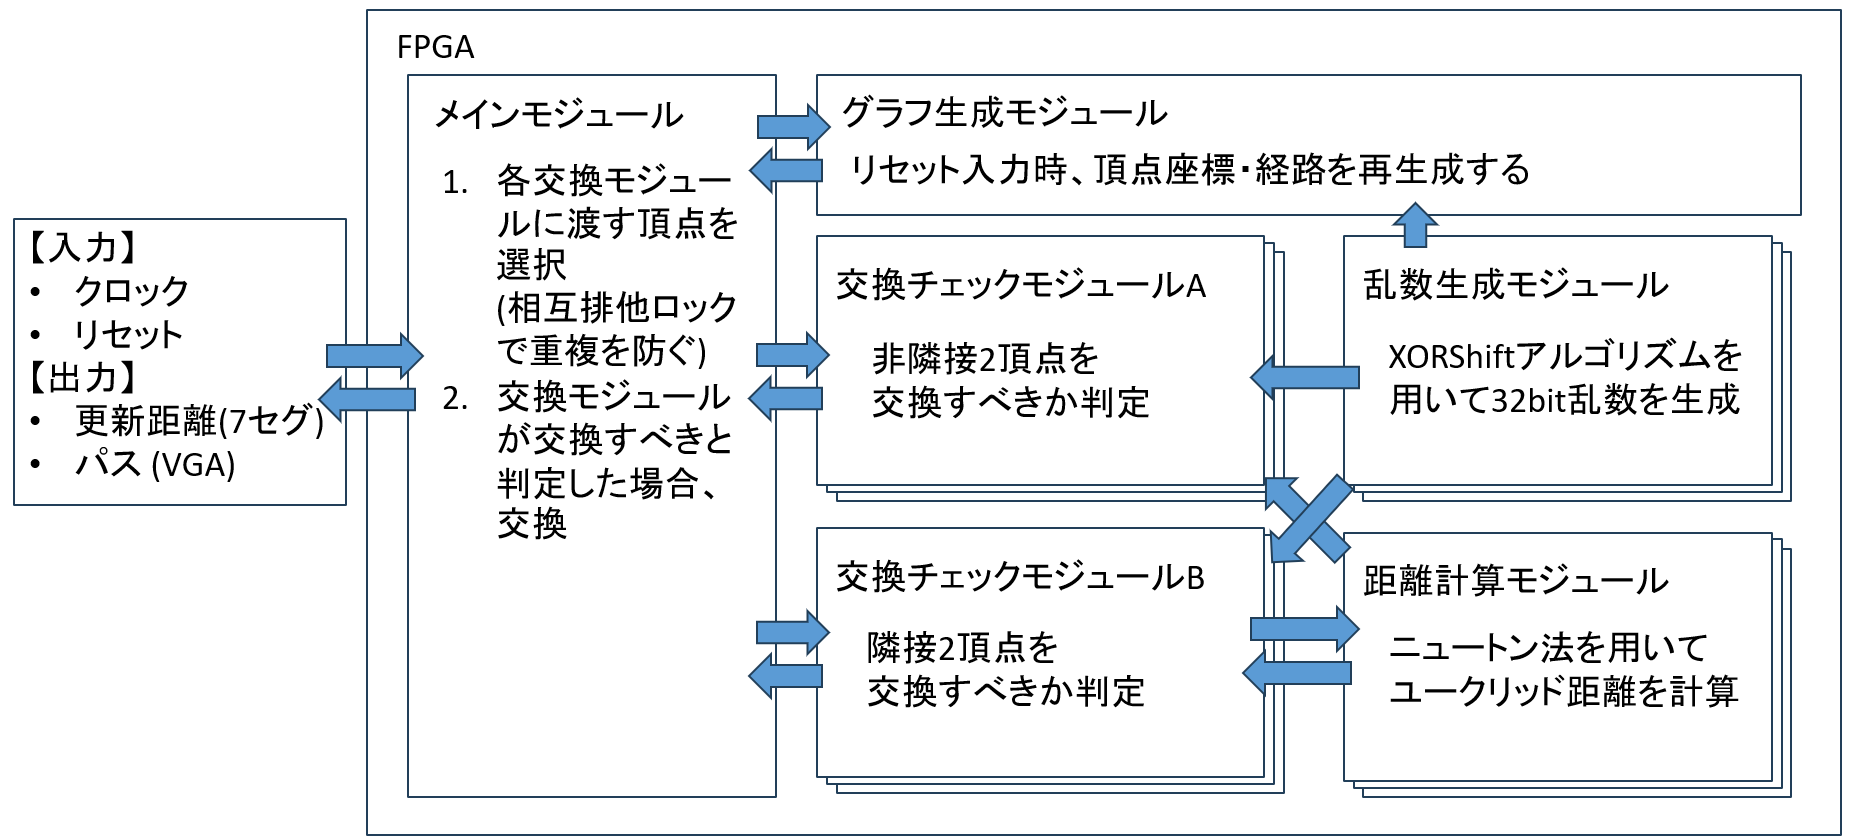
\includegraphics[width=15cm]{figure/hardware.png}
        \caption{ハードウエア構成}
    \end{center}
\end{figure}

図~\ref{fig:hardware}にハードウエアの構成を示す。
FPGAには以下のモジュールを実装した。
\begin{itemize}
    \item メインモジュール(山登り法)
    \item グラフ生成モジュール(近傍生成)
    \item 交換チェックモジュール(交換判定)
    \item 乱数生成モジュール
    \item 距離計算モジュール
\end{itemize}
実行の流れは、
\begin{enumerate}
    \item リセット入力がなされると、グラフ生成モジュールが乱数生成モジュールを用いてランダムな頂点・経路を生成する
    \item メインモジュールが近傍を生成する。
    \item 交換チェックモジュールが距離計算モジュールを用いて交換の有無を判定する。
    \item メインモジュールが交換チェックモジュールからの結果を受け取り、交換の有無に応じて経路を更新する。
    \item 2. に戻る。
\end{enumerate}
である。2. ~ 4. は並列に実行される。

以下では
\begin{enumerate}
    \item 10/23時点での実装内容
    \item 1. の問題点と改善方法
\end{enumerate}
に分けて説明した後、今後の課題について述べる。

\subsection*{乱数生成アルゴリズム}
今回の問題では、ランダムなグラフの生成・近傍の生成など、乱数を用いる箇所が多い。
FPGA上で疑似乱数を生成するためのアルゴリズムとして、今回はXORShiftを用いた。
XORShiftは状態$x, y, z, w$に対し、
\begin{align*}
    x \leftarrow& y \\
    y \leftarrow& z \\
    z \leftarrow& w \\
    w \leftarrow& (w\oplus(w>>19))\oplus((x\oplus(x<<11))\oplus((x\oplus(x<<11))>>8))
\end{align*}
を計算することで疑似乱数列${w}$を求めるアルゴリズムである。
ビット演算のみで計算できるため極めて高速で、また周期も$2^{128}-1$と非常に長く品質も高いという特徴がある。
このアルゴリズムを用いて、クロック毎に新しい乱数を生成するモジュールを作成し、乱数が必要な箇所それぞれでインスタンス化した。

\subsection*{距離計算アルゴリズム}\label{sec:distance}
距離計算モジュールは、2つの頂点のx, y座標$(x_1, y_1), (x_2, y_2)$を受け取り、
2点のユークリッド距離$\sqrt{(x_1-x_2)^2+(y_1-y_2)^2}$を計算するモジュールである。

このモジュールでは、加算減算乗算に加え、平方根の計算が必要となるが、今回はニュートン法を用いて計算した。
ニュートン法において、$\sqrt{a}$の計算のためには、$f(x)=x^2-a$を考える。このとき、$f(x)=0$となる$x$が$\sqrt{a}$である。

解に近い値を初期値$x_0$とし、$x_{n+1}=x_n-\frac{f(x_n)}{f'(x_n)}=x_n-\frac{x_n^2-a}{2x_n}=\frac{x_n}{2}+\frac{a}{2x_n}$に従って$x_n$を更新していくと、
$x_n$は$\sqrt{a}$に収束していく。
今回はユークリッド距離の計算であり、初期値としてマンハッタン距離$d_m=|x_1-x_2|+|y_1-y_2|$を用いると、比較的早く収束する。
x座標、y座標が$[0,255]$の2点に対し、整数範囲で誤差1以内の距離を計算するには、$x_3$まで計算すれば十分であることがCPUプログラムによる検証により判明した。

当初、1クロックで$x_3$までの計算(二乗距離・マンハッタン距離・ニュートン法3回)を実行していたが、後述の通り周波数が大きく低下してしまったため、5クロックに分割しパイプライン化した。

\subsection*{近傍生成アルゴリズム}
\ref{sec:local}節で述べたように、今回は経路の2点を入れ替えることで近傍を生成する。
交換する2点を選ぶには、交換する2点と、それぞれの前後の点の計6点の情報が必要であり、これら6点が重複しないように選択すれば、複数の箇所について同時に近傍を生成し、判定・更新を行うことができる。

各モジュールが頂点を選択する際は、以下の手順で行う
\begin{enumerate}
    \item 乱数生成モジュールから、頂点番号を表す[0,63]の乱数を2つ受け取り、$v_1, v_2$とする。
    \item ロック配列(後述)の$v_1-1, v_1, v_1+1, v_2-1, v_2, v_2+1$番目の要素を確認し、いずれも他のモジュールによってロックされていなければ、ロックを試みる。
    \item 再び$v_1-1, v_1, v_1+1, v_2-1, v_2, v_2+1$番目の要素を確認し、いずれもロックできていれば、交換チェックモジュールに6頂点の座標を送信する。
          一つ以上の頂点がロックに失敗していれば、6頂点すべてのロックを解除し、1. に戻る。
\end{enumerate}
ロック配列は、各頂点が他のモジュールによってロックされているかどうかを表す配列である。(ロックされていなければ-1, ロックされていれば、ロックしているモジュールのIDが格納される。)
この機能によって、複数のモジュールが同時に同じ頂点を選択することを防ぐことができる。
この手法は排他制御ロックと呼ばれており、データベースのトランザクション処理や、マルチスレッドプログラミングにおいてよく用いられる。

\subsection*{交換判定アルゴリズム}
交換判定モジュールは、選択した2頂点(p,q)とその前後の頂点の座標を受け取り、距離計算モジュールを用いて交換するべきかどうか(交換によって総距離が短くなるかどうか)を判定する。

\fbox{パターン1}p,qが隣接していない場合、p, qと前後を含めた6点がa→p→bとc→q→dの順に並んでいるとして、pとqを交換するので、
\begin{itemize}
    \item 交換前: $d(a,p)+d(p,c)+d(d,q)+d(q,f)$
    \item 交換後: $d(a,q)+d(q,c)+d(d,p)+d(p,f)$
\end{itemize}
の2つの距離を計算し、交換後の方が短ければ交換する。

\fbox{パターン2}p,qが隣接している場合、p, qと前後を含めた4点がa→p→q→bの順に並んでいるとして、pとqを交換するので、
\begin{itemize}
    \item 交換前: $d(a,p)+d(p,q)+d(q,f)$
    \item 交換後: $d(a,q)+d(q,p)+d(p,f)$
\end{itemize}
を比較する。$d(p,q)=d(q,p)$より$d(a,p)+d(q,f)$と$d(a,q)+d(p,f)$を計算し、後者の方が小さければ交換する。

山登りモジュールではパターン1とパターン2をそれぞれいくつか用意し、並列度を上げた。

\section*{実験結果}
\subsection*{実装量}
図~\ref{fig:hardware}に示した各モジュールを実装した結果、それぞれのVerilog実装量は以下のようになった。
\begin{table}
    \label{tab:sourcesize}
    \begin{center}
        \caption{各モジュールのVerilog実装量}
            \begin{tabular}{|l|l|l|}
            \hline
            ファイル名                   & 機能                                                                                       & 実装量         \\ \hline\hline
            TSPTop.v   / TSPTop\_wrap.sv & トップモジュール                                                                                 & 40行 +   57行 \\\hline
            Tsp.sv                       & \begin{tabular}[c]{@{}l@{}}・グラフ情報の管理\\・各交換モジュールの呼び出し\\・頂点スワップの実行\end{tabular} & 249行        \\\hline
            Swap.sv                      & 非隣接点交換モジュール                                                                              & 95行         \\\hline
            Swap\_adjacent.sv            & 隣接点交換モジュール                                                                               & 82行         \\\hline
            Graph.sv                     & グラフ生成モジュール                                                                               & 43行         \\\hline
            Distance.v                   & 距離計算モジュール                                                                                & 37行         \\\hline
            Xorshift.v                   & 乱数生成モジュール                                                                                & 25行         \\\hline
            Seg7.sv                      & 7セグ16進出力モジュール                                                                            & 32行         \\\hline\hline
            合計                         &                                                                                          & 約660行      \\\hline
            \end{tabular}
    \end{center}
\end{table}
\subsection*{シミュレーション結果}
PC上でテストベンチを実行し、シミュレーション結果を得た。
シミュレーション結果を図~\ref{fig:sim}に示す。
\begin{figure}[h]
    \label{fig:sim}
    \begin{center}
        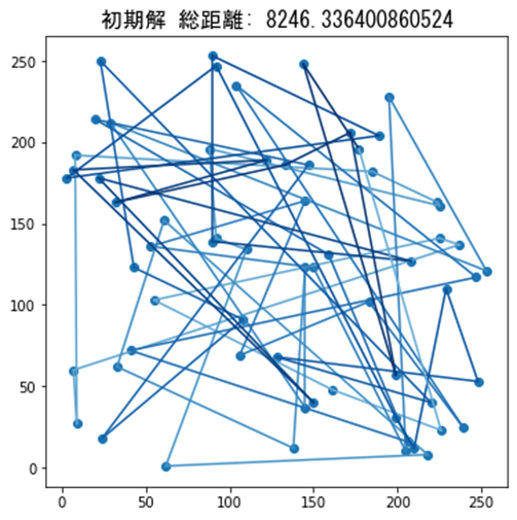
\includegraphics[width=7cm]{figure/fpga_tsp_bad.png}
        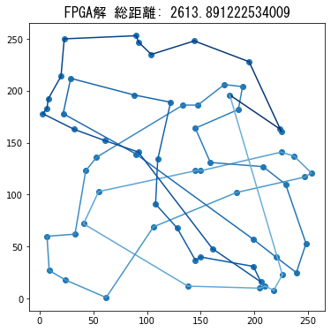
\includegraphics[width=7cm]{figure/fpga_tsp_good.png}
        \caption{シミュレーション結果}
    \end{center}
\end{figure}
リセット入力を与えると、左図のようにランダムなグラフ・経路が生成される。
その後、右図のように山登り法によって経路が更新されていく。最終的には右図のように局所最適解に陥り、今回定めた近傍(パターン1・パターン2)だけではこれ以上改善しない状態になった。

乱数的な手法を用いているため、実行するたびに結果が異なるが、総距離2600~2800程度の局所最適解に陥ることが多かった。
並列度ごとに、局所最適解に陥るまでに要するクロック数を計測した結果を表~\ref{tab:time}に示す。
\begin{table}
    \label{tab:time}
    \begin{center}
        \caption{並列度ごとの局所最適解に陥るまでに要するクロック数}
        \begin{tabular}{|c|c|}
            \hline
            並列度 & 局所最適解に陥るまでに要するクロック数 \\ \hline
            1      & 19.4kクロック                     \\ \hline
            2      & 11.3kクロック                       \\ \hline
            3      & 6.5kクロック                       \\ \hline
        \end{tabular}
    \end{center}
\end{table}
並列度を$n$にすると、局所最適解に陥るまでに要するクロック数は$\frac{1}{n}$になると予想されるが、概ねその通りの結果となった。
\subsection*{合成結果}\label{sec:compile}
Quartus上でコンパイルを行い、並列度ごとに最大周波数・使用ロジック数・使用演算器数を計測した結果を表~\ref{tab:compile}に示す。
\begin{table}
    \label{tab:compile}
    \begin{center}
        \caption{並列度ごとの合成結果}
        \begin{tabular}{|c|c|c|c|}
            \hline
            並列度(パターン1 + パターン2) & 最大周波数 & 使用ロジック数 & 使用演算器数 \\ \hline
            1+0      & 12.76MHz    &  7,470          & 8       \\ \hline
            0+1      & 12.69MHz    &  6,743          & 8       \\ \hline
            1+1      & 12.83MHz    & 14,821          & 16       \\ \hline
            2+1      & 12.73MHz    & 23,152          & 24       \\ \hline
            3+1      & ×           & 50,546          & 32       \\ \hline
        \end{tabular}
    \end{center}
\end{table}
並列度を上げても最大周波数はほとんど変化しなかった。
使用ロジック数は、pow(2, 総並列度)に比例して指数関数的に増加した。並列度4では、使用ロジック数がFPGAのリソースを超えてしまったため、合成に失敗した。
使用演算器数は、総並列度に線形に増加した。

\subsubsection*{ロジックに関する分析}
使用ロジックの内訳として、各交換モジュールは4000程度(うち距離計算が2000程度)しかなく、これらのモジュールを並列につなぎ合わせる部分が使用ロジック数の大きく占めることがわかった。

\subsubsection*{最大動作周波数に関する分析・追加検証}
\ref{sec:distance}節で述べたように、距離計算モジュールは5クロックに分割しパイプライン化した。
当初1クロックで計算していた際、最大周波数が4MHz程度しか出なかったが、5クロックに分割したことで12MHz程度に改善した。
また、ユークリッド距離のかわりにマンハッタン距離を用いた場合、47.8MHzで動作可能であることを確認した。

ステージ分割によって、1クロックあたりの除算の回数が3回から最大1回に減少し、最大動作周波数は三倍程度になった。
このことから、最大動作周波数のボトルネックは距離計算モジュールであり、特に除算に大きな問題があることがわかった。

除算は、加算減算乗算に比べ非常に遅く、一般的なプロセッサでは、数十クロックかけることもある。したがって、除算を含むモジュールは、動作周波数を大きく下げる要因となる。
この問題を是正するために、以下の2つの方法を考え、それぞれ検証した。
\begin{itemize}
    \item 方法1: 除算の高速化
    \item 方法2: 除算を含まない距離計算方法の実装
\end{itemize}
\paragraph*{方法1: 除算の高速化}
今回除算を必要とするのは、二乗距離の平方根を計算する部分であり、各座標が$[0,255]$の8bit整数であることから、二乗距離は18bitで表現可能である。
現状32bitに対する除算を用いていたことから、除算の精度を下げることで高速化を図ることができると考えた。

除算の精度を18bitに下げたところ、最大動作周波数は21.4MHzまで改善した。

\paragraph*{方法2: 除算を含まない距離計算方法の実装}
今回の平方根計算ではニュートン法を用いたが、平方根計算には除算が不要な方法も存在する。
その中でも、二分法を用いて距離計算する方法を検討する。

